% ******************************************************** %
% Copyright © Jonathan Gitlin 2011 – 2013
%
% This work is licensed under the Creative Commons 
% Attribution-NonCommercial-ShareAlike 3.0 Unported License
%
% For More Information See the Creative Commons Website
% http://creativecommons.org
%
% For A human readable summary, See:
% http://creativecommons.org/licenses/by-nc-sa/3.0/
%
% For the Full Text of the License:
% http://creativecommons.org/licenses/by-nc-sa/3.0/legalcode
%
% No Claim Is Made To Original Works 
% Of Other Sources Cited Within This Work
%
% ******************************************************** %

\chapter{Judicial Branch}

\section{Purpose of Chapter}
This chapter covers the Judicial Branch of the United States government, that is, the United States' court system.

\section{Creation}
The Constitution creates the Judicial Branch of the United States in Article III, Section 1:

\begin{quote}
The judicial Power of the United States shall be vested in one supreme Court, and in such inferior Courts as the Congress may from time to time ordain and establish.
\end{quote}

\section{Organization of Judicial Branch}

The Judicial Branch of the United States is organized into three layers, in a hierarchical format.  The Supreme Court sits at the top, with the Courts of Appeals beneath the Supreme Court, and the District Courts beneath the Courts of Appeals.

\subsection{The Supreme Court}
The Supreme Court is the highest court in the United States government and is explicitly created by the Constitution.\footnote{Article III, Section 1 (``The judicial power of the United States, shall be vested in one Supreme Court, and in such inferior courts as the Congress may from time to time ordain and establish.'').}
However, while the Constitution \textit{creates} the Supreme Court, it is silent as to many of the practical details about the Court and its operation.  For example, the Constitution does not establish (1) the number of justices that will sit on the Supreme Court, (2) the time, place, or manner of the Court's meetings, (3) the number of cases that the Court will hear per term, or how those cases will come to be heard by the Court, or (4) the number of justices necessary to establish a quorum for the Court to hold hearings.  Congress has taken the Constitution's silence on these types of matters as an invitation to pass establishing these details about the Court.  Thus, many the Supreme Court's operations and characteristics are set by Congress through federal law.

\subsubsection{Supreme Court Size}

The judges of the Supreme Court are known as ``Justices.''  Per federal law, there are a total of nine Justices that sit on the Supreme Court -- one chief Justice and eight associate Justices.\footnote{28 U.S.C. \S\ 1 (``The Supreme Court of the United States shall consist of a Chief Justice of the United States and eight associate justices, any six of whom shall constitute a quorum.'').}  

However, while the Court currently has nine Justices, the size of the Court has varied over time.  Originally, the Court had six Justices, set by the Judiciary Act of 1789, but over time, the number has fluctuated up and down\footnote{\textit{The Judiciary Act of 1789} (``Sec. 1. Be it enacted, That the supreme court of the United States shall consist of a chief justice and five associate justices, any four of whom shall be a quorum, and shall hold annually at the seat of government two sessions''); 

\textit{The Judiciary Act of 1801}, 2 Stat. 89, February 13, 1801 (``SEC. 3. And be it further enacted, That from and after the next vacancy that shall happen in the said court, it shall consist of five justices only; that is to say, of one chief justice, and four associate justices.''); 

Repeal of \textit{The Judiciary Act of 1801} on March 8, 1802; 

\textit{Act Establishing the Seventh Circuit}, 2 Stat. 420, February 24, 1807 (``SEC. 5. Be it further enacted, That the supreme court of the United States shall hereafter consist of a chief justice, and six associate justices, any law to (the) contrary notwithstanding.''); 

\textit{Act Establishing the Eighth and Ninth Circuits}, 5 Stat. 176, March 3, 1837 (``Be it enacted, by the Senate and House of Representatives of the United States of America in Congress assembled, That the Supreme Court of the United States shall hereafter consist of a chief justice, and eight associate judges, any five of whom shall constitute a quorum;''); 

\textit{Act Establishing the Tenth Circuit}, 12 Stat. 794, March 3, 1863 (``Be it enacted by the Senate and House of Representatives of the United States of America in Congress assembled, That the supreme court of the United States shall hereafter consist of a chief justice and nine associate justices, any six of whom shall constitute a quorum;'');

\textit{Reorganization of the Judicial Circuits}, 14 Stat. 209, 14 Stat. 209 (``Be it enacted by the Senate and House of Representatives of the United States of America in Congress assembled, That no vacancy in the office of associate justice of the supreme court shall be filled by appointment until the number of associate justices shall be reduced to six; and thereafter the said supreme court shall consist of a chief justice of the United States and six associate justices, any four of whom shall be a quorum;'');

\textit{The Judiciary Act of 1869}, 16 Stat. 44, April 10, 1869 (``Be it enacted by the Senate and House of Representatives of the United States of America in Congress assembled, That the Supreme Court of the United States shall hereafter consist of the Chief Justice of the United States and eight associate justices, any six of whom shall constitute a quorum;'')

}:

\begin{center}
  \begin{tabular}{ | c | c | }
   \hline 
	\raisebox{-1.0ex}{\begin{large} \textbf{Year} \end{large}} & \raisebox{-1.0ex}{\begin{large} \textbf{Number of Justices} \end{large}} \\ [1ex] \hline
1789 & 6 \\ \hline
1801 & 5 \\ \hline
1802 & 6 \\ \hline
1807 & 7  \\ \hline
1837 & 9 \\ \hline
1863 & 10 \\ \hline
1866 & 7  \\ \hline
1869 & 9  \\ \hline
  \end{tabular}
\end{center}

In 1869 Congress passed \textit{The Judiciary Act of 1869} which set the number of Justices at nine and it has stayed the same ever since.

\subsubsection{Chief Justice and Associate Justices}
Like the various acts before it, \textit{The Judiciary Act of 1869} set the number of Justices on the Court by specifying a particular number of associate Justices and one Chief Justice.\footnote{\textit{The Judiciary Act of 1869}, 16 Stat. 44, April 10, 1869 (``the Supreme Court of the United States shall hereafter consist of the Chief Justice of the United States and eight associate justices'').}
The Chief and the associate Justices are all equal members of the Court.  However, by tradition the Chief Justice is informally referred to as the ``first among equals.''

Because the Chief Justice and the Associate Justices all have equal votes in the Court's decision-making process, the Chief Justice does not hold any special voting privileges when the Court decides cases.  However, as the chief, the Chief Justice holds certain privileges and responsibilities.  For example, as described in more detail below, the Chief enjoys a preemptive seniority status in assigning opinions when the Court decides a case.  Further, the Chief has various administrative tasks such as being a member of the Board of Regents of the Smithsonian and presiding over the United States Judicial Conference.\footnote{20 U.S.C. \S\ 42(a)(``The business of the Institution shall be conducted at the city of Washington by a Board of Regents, named the Regents of the Smithsonian Institution, to be composed of the Vice President, the Chief Justice of the United States, three Members of the Senate, three Members of the House of Representatives, and nine other persons, other than Members of Congress, two of whom shall be resident in the city of Washington, and seven of whom shall be inhabitants of some State, but no two of them of the same State.''); 28 U.S.C. \S\ 331 (``The Chief Justice of the United States shall summon annually the chief judge of each judicial circuit, the chief judge of the Court of International Trade, and a district judge from each judicial circuit to a conference at such time and place in the United States as he may designate. He shall preside at such conference which shall be known as the Judicial Conference of the United States.'').}

\subsubsection{Terms and Quorum Size}
By federal law, the Supreme Court's term  begins on the first Monday in October each year, and continues until the Court adjourns.\footnote{28 USC \S\ 2 (``The Supreme Court shall hold at the seat of government a term of court commencing on the first Monday in October of each year and may hold such adjourned or special terms as may be necessary.'').}
Six Justices are required for a quorum to hear and decide cases.\footnote{28 U.S.C. \S\ 1 (``The Supreme Court of the United States shall consist of a Chief Justice of the United States and eight associate justices, any six of whom shall constitute a quorum.'').}  


\subsection{Circuit Courts of Appeals}
While Article III explicitly creates the Supreme Court, it leaves the creation of all inferior Courts to Congress.\footnote{Article III, Section 1 (``The judicial power of the United States, shall be vested in one Supreme Court, and in such inferior courts as the Congress may from time to time ordain and establish.'').}
All of the Courts beneath the Supreme Court (i.e. the ``inferior courts'' referred to in Article III) are created and governed by Title 28 of the United States Code.  Immediately below the Supreme Court in the hierarchy of the United States Judiciary are the Courts of Appeals.  The Courts of Appeals are divided up into ``Circuits,'' which for the most part encompass geographical regions.  

Federal law establishes the following Circuits with the specified areas of composition\footnote{28 U.S.C. \S\ 41 (``The thirteen judicial circuits of the United States are constituted as follows: ... District of Columbia	District of Columbia. First	Maine, Massachusetts, New Hampshire, Puerto Rico, Rhode Island. Second	Connecticut, New York, Vermont. Third	Delaware, New Jersey, Pennsylvania, Virgin Islands. Fourth	Maryland, North Carolina, South Carolina, Virginia, West Virginia. Fifth	District of the Canal Zone, Louisiana, Mississippi, Texas. Sixth	Kentucky, Michigan, Ohio, Tennessee.
Seventh	Illinois, Indiana, Wisconsin. Eighth	Arkansas, Iowa, Minnesota, Missouri, Nebraska, North Dakota, South Dakota. Ninth	Alaska, Arizona, California, Idaho, Montana, Nevada, Oregon, Washington, Guam, Hawaii. Tenth	Colorado, Kansas, New Mexico, Oklahoma, Utah, Wyoming. Eleventh	Alabama, Florida, Georgia. Federal	All Federal judicial districts.'').} :

\begin{center}
  \begin{tabular}{ | l | p{8cm} | }
   \hline 
    \raisebox{-1.0ex}{\begin{large} \textbf{Circuit} \end{large}} & \raisebox{-1.0ex}{\begin{large} \textbf{Composition} \end{large}} \\ [1ex] \hline

First & Maine, Massachusetts, New Hampshire, Puerto Rico, Rhode Island.\\ \hline
Second & Connecticut, New York, Vermont.\\ \hline
Third & Delaware, New Jersey, Pennsylvania, Virgin Islands.\\ \hline
Fourth & Maryland, North Carolina, South Carolina, Virginia, West Virginia.\\ \hline
Fifth & District of the Canal Zone, Louisiana, Mississippi, Texas.\\ \hline
Sixth & Kentucky, Michigan, Ohio, Tennessee.\\ \hline
Seventh & Illinois, Indiana, Wisconsin.\\ \hline
Eighth & Arkansas, Iowa, Minnesota, Missouri, Nebraska, North Dakota, South Dakota.\\ \hline
Ninth & Alaska, Arizona, California, Idaho, Montana, Nevada, Oregon, Washington, Guam, Hawaii.\\ \hline
Tenth & Colorado, Kansas, New Mexico, Oklahoma, Utah, Wyoming.\\ \hline
Eleventh & Alabama, Florida, Georgia.\\ \hline
District of Columbia & District of Columbia.\\ \hline
Federal & All Federal judicial districts.\\ \hline

  \end{tabular}
\end{center}

Each of the specified circuits has a corresponding Circuit Court of Appeals.\footnote{28 U.S.C. \S\ 43(a) (``There shall be in each circuit a court of appeals, which shall be a court of record, known as the United States Court of Appeals for the circuit.'').}  The Courts of Appeals handle all of the appeals from the lower courts comprising their respective circuit.

\subsection{District Courts}
Beneath the Courts of Appeals are the District Courts, which are the United States' trial courts.  The United States' District Courts handle the vast majority of the federal trial work in the United States and perform the functions that most people generally think of as a ``trial.''


\subsubsection{Districts}
Just as the Judicial Branch is divided up into Circuits at the Court of Appeals level, the Judiciary is further subdivided into Districts at the trial court level.\footnote{See Chapter 5 of Title 28, Sections 81 -- 131:  \S\ 81. Alabama, \S\ 81A. Alaska, \S\ 82. Arizona, \S\ 83. Arkansas, \S\ 84. California, \S\ 85. Colorado, \S\ 86. Connecticut, \S\ 87. Delaware, \S\ 88. District of Columbia, \S\ 89. Florida, \S\ 90. Georgia, \S\ 91. Hawaii, \S\ 92. Idaho, \S\ 93. Illinois, \S\ 94. Indiana, \S\ 95. Iowa, \S\ 96. Kansas, \S\ 97. Kentucky, \S\ 98. Louisiana, \S\ 99. Maine, \S\ 100. Maryland, \S\ 101. Massachusetts, \S\ 102. Michigan, \S\ 103. Minnesota, \S\ 104. Mississippi, \S\ 105. Missouri, \S\ 106. Montana, \S\ 107. Nebraska, \S\ 108. Nevada, \S\ 109. New Hampshire, \S\ 110. New Jersey, \S\ 111. New Mexico, \S\ 112. New York, \S\ 113. North Carolina, \S\ 114. North Dakota, \S\ 115. Ohio, \S\ 116. Oklahoma, \S\ 117. Oregon, \S\ 118. Pennsylvania, \S\ 119. Puerto Rico, \S\ 120. Rhode Island, \S\ 121. South Carolina, \S\ 122. South Dakota, \S\ 123. Tennessee, \S\ 124. Texas, \S\ 125. Utah, \S\ 126. Vermont, \S\ 127. Virginia, \S\ 128. Washington, \S\ 129. West Virginia, \S\ 130. Wisconsin, \S\ 131. Wyoming.}  
Like the Circuits, the Districts, for the most part, encompass geographical regions -- each District is a subdivision of a particular Circuit and encompasses either a State or a smaller portion thereof.

So, for example, while the Fifth Circuit may comprise all of Louisiana, Mississippi, and Texas, the State of Texas is divided up into four United States Districts -- the Northern District of Texas, the Southern District of Texas, the Eastern District of Texas, and the Western District of Texas.\footnote{28 USC \S\ 124 (``Texas is divided into four judicial districts to be known as the Northern, Southern, Eastern, and Western Districts of Texas.'').}

\subsubsection{Divisions}
Further, Districts are themselves subdivided into \textit{Divisions}, each Division encompassing a smaller geographical region of its parent District.  So, for example, while the State of Texas is divided up into four United States Districts, the Northern District of Texas is itself subdivided into seven Divisions: (1) The Dallas Division, (2) The Fort Worth Division, (3) The Abilene Division, (4) The San Angelo Division, (5) The Amarillo Division, (6) The Wichita Falls Division, and (7) The Lubbock Division.\footnote{28 USC \S\ 124(a) (``The Northern District comprises seven divisions.  (1) The Dallas Division comprises the counties of Dallas, Ellis, Hunt, Johnson, Kaufman, Navarro, and Rockwall.  Court for the Dallas Division shall be held at Dallas.  (2) The Fort Worth Division comprises the counties of Comanche, Erath, Hood, Jack, Palo Pinto, Parker, Tarrant, and Wise.  Court for the Fort Worth Division shall be held at Fort Worth.  (3) The Abilene Division comprises the counties of Callahan, Eastland, Fisher, Haskell, Howard, Jones, Mitchell, Nolan, Shackleford, Stephens, Stonewall, Taylor, and Throckmorton.  Court for the Abilene Division shall be held at Abilene.  (4) The San Angelo Division comprises the counties of Brown, Coke, Coleman, Concho, Crockett, Glasscock, Irion, Menard, Mills, Reagan, Runnels, Schleicher, Sterling, Sutton, and Tom Green.  Court for the San Angelo Division shall be held at San Angelo.  (5) The Amarillo Division comprises the counties of Armstrong, Brisco, Carson, Castro, Childress, Collingsworth, Dallam, Deaf Smith, Donley, Gray, Hall, Hansford, Hartley, Hemphill, Hutchinson, Lipscomb, Moore, Ochiltree, Oldham, Parmer, Potter, Randall, Roberts, Sherman, Swisher, and Wheeler.  Court for the Amarillo Division shall be held at Amarillo.  (6) The Wichita Falls Division comprises the counties of Archer, Baylor, Clay, Cottle, Foard, Hardeman, King, Knox, Montague, Wichita, Wilbarger, and Young.  Court for the Wichita Falls Division shall be held at Wichita Falls.  (7) The Lubbock Division comprises the counties of Bailey, Borden, Cochran, Crosby, Dawson, Dickens, Floyd, Gaines, Garza, Hale, Hockley, Kent, Lamb, Lubbock, Lynn, Motley, Scurry, Terry, and Yoakum.  Court for the Lubbock Division shall be held at Lubbock.'').}

Ultimately, each District Court sits in particular geographical location and is referred to by its District and Division, such as a District Court for the Dallas Division of the Northern District of Texas.

\subsubsection{Number of District Courts}
The number of District Courts is set by federal law.\footnote{See 28 USC \S\ 133(a).}  For example, 28 USC \S\ 133(a) establishes that in Texas the Northern District has twelve District Courts, the Southern District has nineteen District Courts, the Eastern District has seven District Courts, and the Western District has thirteen District Courts.\footnote{28 USC \S\ 133(a) (``The President shall appoint, by and with the advice and consent of the Senate, district judges for the several judicial districts, as follows: ... Texas: Northern 12 Southern 19  Eastern 7 Western 13'').}






\section{Judges}
Judges are the core of the United States Judicial Branch.  They sit on the courts and conduct the business of the United States Judicial Branch.  


\subsection{Nomination and Confirmation of Judges}
United States judges become United States judges through a nomination and confirmation process; the President nominates a judge, and the Senate must confirm the President's nomination.  The process is the same for all levels of the Judiciary, from the Supreme Court all the way down to the District Courts.  The nomination and confirmation process is established by the Constitution for Supreme Court Justices and by Federal law for all lower Court judges.\footnote{Article II, Section 2 (``he shall nominate, and by and with the Advice and Consent of the Senate, shall appoint Ambassadors, other public Ministers and Consuls, Judges of the supreme Court, and all other Officers of the United States, whose Appointments are not herein otherwise provided for, and which shall be established by Law''); 28 U.S.C. \S\ 44(a) (``The President shall appoint, by and with the advice and consent of the Senate, circuit judges for the several circuits.''); 28 U.S.C. \S\ 133(a) (``The President shall appoint, by and with the advice and consent of the Senate, district judges for the several judicial districts'').}


\subsection{Separation of Powers}
As covered in more depth below, the Judicial Branch is the weakest of the three branches of government.\footnote{Federalist \#78 (``It proves incontestably, that the judiciary is beyond comparison the weakest of the three departments of power;'')}  Therefore, to secure the Judiciary from incursion or control by the other two branches (and accordingly to protect the separation of powers in the United States' government), the Constitution establishes two vital protections that apply to all United States Judges, from the Supreme Court Justices all the way down to the District Courts Judges:

\begin{enumerate}
\item \textbf{Life Tenure}  First, the Constitution establishes that all Judges in the United States Judicial Branch have life tenure.  Article III, Section 1, provides that ``The Judges, both of the supreme and inferior Courts, shall hold their Offices during good Behaviour.''  In other words, once United States Judges are nominated and confirmed they do not have any set terms limits.  Once ``in office'' the Judges do not need to be renominated or reconfirmed to remain in their position as a United States judge.  

However, per Article I, Congress can still involuntarily remove a Judge from office through the impeachment and conviction process.\footnote{See the previous chapter on the Legislative Branch for a more detailed explanation of this process.}  This is, however, a rare occurrence because it requires an impeachment by the House of Representatives and conviction by the Senate.  Thus, short of retirement or death, it literally takes an act of Congress to remove a United States Judge from office.  

In the Federalist \#78, Alexander Hamilton explains how this protects the separation of powers in the United States government:

\begin{quote}
That inflexible and uniform adherence to the rights of the Constitution, and of individuals, which we perceive to be indispensable in the courts of justice, can certainly not be expected from judges who hold their offices by a temporary commission. Periodical appointments, however regulated, or by whomsoever made, would, in some way or other, be fatal to their necessary independence. If the power of making them was committed either to the Executive or legislature, there would be danger of an improper complaisance to the branch which possessed it; if to both, there would be an unwillingness to hazard the displeasure of either; if to the people, or to persons chosen by them for the special purpose, there would be too great a disposition to consult popularity, to justify a reliance that nothing would be consulted but the Constitution and the laws.
\end{quote}

Hamilton begins by highlighting the importance of having a separate and independent Judicial Branch -- the Judicial Branch protects the rights of the Constitution and people of the United States from encroachment by the other two branches.  Hamilton then points out that this ''inflexible and uniform adherence'' to the Constitution in defiance of attempts by the other branches to ignore or invade protected rights cannot be expected from judges that have only a temporary commission and rely on either or both of the other two branches for their continued employment.  Having to rely on another branch for continuing employment would create in judges ``an unwillingness to hazard the displeasure'' of the other branch upon which they relied for their reappointment.

Thus, according to Hamilton, life tenure gives the Judges of the United States Judicial Branch an independence that stands as an ``excellent barrier to the encroachments and oppressions'' by the other two branches and secures ``a steady, upright, and impartial administration of the laws.''\footnote{Federalist \#78.}

\item \textbf{Salary Protection}  The second protection that the Constitution provides to the Judicial Branch is salary protection.  Alexander Hamilton summarizes the importance of this protection in the Federalist \#78:
\begin{quote}
a power over a man's subsistence amounts to a power over his will. And we can never hope to see realized in practice, the complete separation of the judicial from the legislative power, in any system which leaves the former dependent for pecuniary resources on the occasional grants of the latter
\end{quote}

Hamilton says, succinctly, that the power over a man's purse is the power over his will.  And because the Judges of the Judicial Branch are dependent on Congress for their salaries, the Judiciary cannot truly be an independent branch of the government in practice without salary protection to prevent coercion by Congress.  Thus, Article I, Section 3 of the Constitution provides: 

\begin{quote}
The Judges, both of the supreme and inferior Courts ... shall, at stated Times, receive for their Services a Compensation, which shall not be diminished during their Continuance in Office.
\end{quote}

Thus, a Judge's salary cannot be reduced while the Judge is in office.  Accordingly, Congress is always free to raise Judges' salaries, but once raised they cannot reduce them.

\end{enumerate}




\section{Power of Judiciary}

The power of the Judicial Branch is the power of the United States Courts to hear and decide cases.  A court's ability to hear and decide a case is known as its ``jurisdiction,'' and the scope of a court's jurisdiction is the range of subject matters that the court can adjudicate.  


Just as State Governments and the Federal Government have fundamentally different presumptions regarding their power as a whole, State Courts and Federal Courts have fundamentally different presumptions regarding their jurisdiction (i.e. their ability to hear and decide cases).  

State governments are intended to be general-purpose governments and are presumed to have power absent a specific restriction.  Similarly, State Courts are intended to be general-purpose courts and are presumed to have judicial power to adjudicate a dispute absent a specific restriction.
State Courts are referred to as courts of \textit{general} jurisdiction and handle the vast majority of all the lawsuits in the United States.

Alternatively, Federal Courts operate from the opposite premise.  The Federal Government is a limited-purpose government, and can only exercise that power specifically authorized by the Constitution.  Similarly, Federal Courts are limited-purpose Courts, and can only exercise judicial power as authorized by the Constitution.  Because of this, Federal Courts are courts of \textit{limited} jurisdiction.  A Federal Courts is presumed to lack jurisdiction to adjudicate a dispute that comes before it and the burden of establishing the contrary rests upon the party asserting jurisdiction.\footnote{Kokkonen v. Guardian Life Ins. Co. of America, 511 U. S. 375, 377 (1994)(``Federal courts are courts of limited jurisdiction ... It is to be presumed that a cause lies outside this limited jurisdiction ... and the burden of establishing the contrary rests upon the party asserting jurisdiction'').}



\subsection{Constitutional Limits of Judicial Power}
Article III, Section 2 of the Constitution establishes the \textit{maximum} scope of the Judicial Power of the United States government:

\begin{quote}

The judicial Power shall extend to all Cases, in Law and Equity, arising under this Constitution, the Laws of the United States, and Treaties made, or which shall be made, under their Authority;--to all Cases affecting Ambassadors, other public Ministers and Consuls;--to all Cases of admiralty and maritime Jurisdiction;--to Controversies to which the United States shall be a Party;--to Controversies between two or more States;-- between a State and Citizens of another State,--between Citizens of different States,--between Citizens of the same State claiming Lands under Grants of different States, and between a State, or the Citizens thereof, and foreign States, Citizens or Subjects.\footnote{Parts of this are altered by the Eleventh Amendment}

\end{quote}

Succinctly, this gives the Judicial Branch judicial power over, \textit{at most}, the following categories of disputes:
\begin{itemize}
\item The United States' Constitution, laws, and treaties
\item Ambassadors
\item Admiralty Cases (cases involving events occurring at sea)
\item Cases by or against the United States
\item When one state sues another state
\item When a person from one state sues a person from another state
\item Cases involving land grants by different states
\item Cases involving foreign states or their citizens
\end{itemize}

Thus, for example, if a Texas citizen wanted to sue another Texas citizen for a cause of action based solely on Texas state law (such as breach of contract), the general rule is that the United States could not decide the case.  The Constitution does not authorize the United States Judicial Branch to resolve disputes between two citizens of the same State where the claims are based wholly on state law.\footnote{This is a general rule, though, and circumstances do exist (e.g. bankruptcy cases) where the United States may resolve wholly intrastate disputes.} Thus, such a case would fall outside of the grant of judicial power by the Constitution to the Judiciary and the United States Judicial Branch would not be authorized to exercise jurisdiction over such a case.

\subsection{Statutory Boundaries of Judicial Power}

As covered above, the Constitution defines the \textit{limits} of the United States government's judicial power.  It does not, however, actually \textit{create} jurisdiction for the United States Courts to hear cases.\footnote{Except in a few limited cases.}
Instead, the Constitution assigns the power to create the Judiciary's jurisdiction to the Legislative Branch, so long as Congress' definition of the courts' jurisdiction fits within the boundaries established by the Constitution.

As an analogy, consider two boxes, one contained within another:

\begin{center}
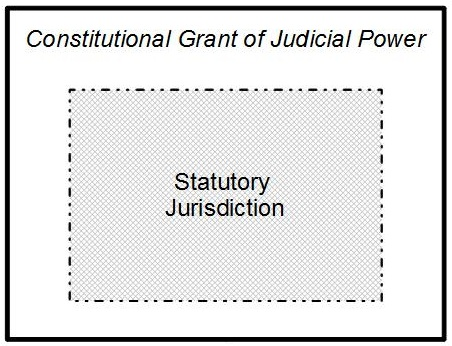
\includegraphics[scale=0.5]{jxboundaries.jpg}
\end{center}

The outer box is the limit of the United States' judicial power, as established by the Constitution.  It sets the absolute boundaries of the judicial power that United States Courts can exercise.  The inner box is the \textit{actual} jurisdiction of the United States' Courts as authorized by Congress.  

Congress can expand or contract the inner box (the actual jurisdiction of the United States Courts) as it sees fit, but the size and scope of the inner box must always be less than or equal to the size and scope of the outer box; the inner box can never be larger than the outer box (i.e. the jurisdiction authorized by Congress can never exceed the boundaries on the judicial power of the United States government established by the Constitution.)


This is the relationship between the Constitutional grant of Judicial Power and the statutory limits of the United States Courts' jurisdiction as set by federal law.


\subsubsection{Statutory Jurisdiction of United States Courts}


Title 28 of the United States Code, Sections 1251 -- 1631, defines the jurisdiction of United States courts, from the Supreme Court all the way down to the District Courts.



At the trial court level, litigants most often use 28 U.S.C. \S\ 1331 and 28 U.S.C. \S\ 1332 to establish Federal jurisdiction to gain access to Federal District Courts.

\subsubsection{28 U.S.C. \S\ 1331 -- Federal Question Jurisdiction}  28 U.S.C. \S\ 1331 grants District Courts jurisdiction to hear and decide cases involving the Constitution, laws, or treaties of the United States:

\begin{quote}
The district courts shall have original jurisdiction of all civil actions arising under the Constitution, laws, or treaties of the United States.
\end{quote}

This is known as ``federal question'' jurisdiction because it authorizes United States District Courts to hear and decide cases concerning ``federal questions'' - i.e. cases or controversies dealing with the United States' (1) Constitution, (2) laws, and (3) treaties.\footnote{
\textit{Mims v. Arrow Financial Services, LLC}, 132 S. Ct. 740, 744 (2012)(``Mims invoked the court's ``federal question'' jurisdiction, i.e., its authority to adjudicate claims ``arising under the ... laws ... of the United States,'' 28 U.S.C. § 1331'').}

As for the Constitutionality of this jurisdictional grant, Congress is within its power to grant the District Courts jurisdiction to hear and decide ``federal question'' cases because Article III, Section 2 of the Constitution extends the judicial power of the United States to ``all Cases, in Law and Equity, arising under this Constitution, the Laws of the United States, and Treaties made.''\footnote{Article III, Section 2 (``The judicial Power shall extend to all Cases, in Law and Equity, arising under this Constitution, the Laws of the United States, and Treaties made, or which shall be made, under their Authority;--to all Cases affecting Ambassadors, other public Ministers and Consuls;--to all Cases of admiralty and maritime Jurisdiction;--to Controversies to which the United States shall be a Party;--to Controversies between two or more States;-- between a State and Citizens of another State,--between Citizens of different States,--between Citizens of the same State claiming Lands under Grants of different States, and between a State, or the Citizens thereof, and foreign States, Citizens or Subjects.'').}  Thus, Congress has not exceeded the bounds on the United States' judicial power established by the Constitution by granting District Courts jurisdiction to hear and decide federal question cases (i.e. the ``inner box'' from the diagram above has not been made to exceed the size of the ``outer box.'').

\subsubsection{28 U.S.C. \S\ 1332 -- Diversity Jurisdiction} 
28 U.S.C. \S\ 1332 grants District Courts jurisdiction to hear and decide cases involving citizens of different states or foreign states, so long as the amount in controversy exceeds a required minimum dollar amount:

\begin{quote}
The district courts shall have original jurisdiction of all civil actions where the matter in controversy exceeds the sum or value of \$75,000, exclusive of interest and costs, and is between—
\begin{enumerate}
\item citizens of different States;
\item citizens of a State and citizens or subjects of a foreign state;
\item citizens of different States and in which citizens or subjects of a foreign state are additional parties; and
\item a foreign state, defined in section 1603 (a) of this title, as plaintiff and citizens of a State or of different States.
\end{enumerate}
\end{quote}

This is known as ``diversity jurisdiction'' because it authorizes United States District Courts to hear and decide cases between residents of different states or foreign states (i.e. the litigants have ``diversity'' of State residences), so long as the amount in controversy is over \$75,000.00.

As for the Constitutionality of this jurisdictional grant, Congress is within its power to grant the District Court jurisdiction to hear and decide ``diversity jurisdiction'' cases because Article III, Section 2 of the Constitution extends the judicial power of the United States to ``to Controversies ... between Citizens of different States.''\footnote{Article III, Section 2 (``The judicial Power shall extend to all Cases, in Law and Equity, arising under this Constitution, the Laws of the United States, and Treaties made, or which shall be made, under their Authority;--to all Cases affecting Ambassadors, other public Ministers and Consuls;--to all Cases of admiralty and maritime Jurisdiction;--to Controversies to which the United States shall be a Party;--to Controversies between two or more States;-- between a State and Citizens of another State,--between Citizens of different States,--between Citizens of the same State claiming Lands under Grants of different States, and between a State, or the Citizens thereof, and foreign States, Citizens or Subjects.'').}  Thus, Congress has not exceeded the bounds on the United States' judicial power established by the Constitution by granting District Courts jurisdiction to hear and decide diversity cases (i.e. the ``inner box'' from the diagram above has not been made to exceed the size of the ``outer box.'').


\subsubsection{Example Case}

Consider a case where a Texas citizen wants to sue another Texas citizen for a cause of action based solely on state law.  Because the litigant's claims are purely state-law claims and both parties are citizens of the same state, the United States District Court would not be authorized to hear and decide the case under either the federal question or diversity jurisdiction statutes.

However, suppose instead that a Texas citizen wants to sue an Oklahoma citizen for \$100,000.00 based solely on a state-law cause of action (such as breach of contract).  Now, a United States District Court \underline{could} hear and decide the case, because there is proper \textit{statutory} jurisdiction under 28 U.S.C. \S\ 1332 because (1) the two parties are citizens of different states and (2) amount in controversy (\$100,000.00) exceed the required statutory minimum (\$75,000.00) and, as covered above, Congress' grant of diversity jurisdiction does not exceed the bounds on the United States' judicial power established by the Constitution.


\section{Exercise of Judicial Power}


Practically speaking, a United States Court exercises the judicial power of the United States by hearing and deciding cases that come before it.
Typically, when deciding a case, a Court considers the evidence of the parties, the argument of counsel, and the law as applicable to the case, and renders a decision based on its consideration of the same.  

Sometimes, a Court will write an opinion detailing the reasoning behind its decision, and when a court does this it typically has a two-fold effect.  First, the Court's opinion informs the parties for the immediate case of both the Court's decision as well as the Court's reasoning behind its decision.  Second, the Court's opinion carries forward through a system known as ``common law,'' and as detailed below, influences how subsequent cases are decided by other Courts in the future.


\subsection{Common Law}

There are, generally speaking, two types of law -- statutory law and common law.  Statutory law is law made by a legislative body, such as Congress.  A law passed by a legislature is called a ``statute'' and the body of law comprising these statutes is known as statutory law.

In contrast, common law is the body of opinions written by the courts.  As mentioned above, common law is based around the premise that when a Court decides a case, it influences how future cases are decided.  The principle behind this is that Courts should decide similar cases similarly.  

For example, suppose that Person A \& Person B come into a court with a dispute.  Suppose that it is important to the parties' dispute that A has 5 widgets and B has 2 gadgets.  After considering the facts of the case, the court decides in favor of A, based on the number of widgets A has versus the number of gadgets B has.  Now, suppose that Person C \& Person D next come in to court with the same dispute, and C \& D have the same number of widgets and gadgets between them that A \& B had.  Because the court decided the first case in A's favor based on the number of widgets A owned, the court should reach a similar decision in C's favor based on the number of widgets C owns.  This is based on the common law premise that when a Court is faced with similar controversies it should reach similar outcomes.

Thus, because future courts will refer to and be influenced in their decisions by past cases in the same way that they refer to and are influenced in their decisions by statutes, common law has the same practical effect as statutory law.



\subsection{Declaring a Statute Unconstitutional}

So which has precedence -- statutory law or common law?  The general rule is that statutory law trumps common law, and when in conflict Courts will give precedence to a statute.
However, what happens when a Court runs into a statute that is contrary to the Constitution?  
Both the Constitution and the statute are law, but when the two are in conflict one must trump the other.
So how does a Court decide which to give precedence to?
Alexander Hamilton discussed this in the Federalist \#78:

\begin{quote}

By a limited Constitution, I understand one which contains certain specified exceptions to the legislative authority; 
such, for instance, as that it shall pass no bills of attainder, no ex post facto laws, and the like. 
Limitations of this kind can be preserved in practice no other way than through the medium of courts of justice, whose duty it must be to declare all acts contrary to the manifest tenor of the Constitution void. 
Without this, all the reservations of particular rights or privileges would amount to nothing ...

There is no position which depends on clearer principles, than that every act of a delegated authority, contrary to the tenor of the commission under which it is exercised, is void. 
No legislative act, therefore, contrary to the Constitution, can be valid. To deny this, would be to affirm, that the deputy is greater than his principal; that the servant is above his master; that the representatives of the people are superior to the people themselves; that men acting by virtue of powers, may do not only what their powers do not authorize, but what they forbid.

\end{quote}

While the Constitution delegates legislative authority to Congress, this delegation is limited to a specific set of enumerated powers.  As such, in order to be valid, an exercise of legislative power by Congress must be contained within the bounds established by the Constitution.  Otherwise such act is without Constitutional validity, because, per Hamilton, ``every act of a delegated authority, contrary to the tenor of the commission under which it is exercised, is void.''  Thus, ``[n]o legislative act ... contrary to the Constitution, can be valid.''  Accordingly, any statute that contradicts the Constitution must yield to the Constitution, and whenever a Court encounters a conflict between a statute and the Constitution, and Court must give the Constitution precedence over the statute.


The United States Supreme Court took up this issue at the turn of the 19th Century in the famous \textit{Marbury v. Madison} case.\footnote{Marbury v. Madison, 5 US 137 (1803).}

\begin{quote}

To what purpose are powers limited, and to what purpose is that limitation committed to writing, if these limits may, at any time, be passed by those intended to be restrained? 

The distinction between a government with limited and unlimited powers is abolished, if those limits do not confine the persons on whom they are imposed, and if acts prohibited and acts allowed, are of equal obligation. 

It is a proposition too plain to be contested, that the constitution controls any legislative act repugnant to it; or, that the legislature may alter the constitution by an ordinary act.

Between these alternative there is no middle ground. The constitution is either a superior paramount law, unchangeable by ordinary means, or it is on a level with ordinary legislative acts, and, like other acts, is alterable when the legislature shall please to alter it.

If the former part of the alternative be true, then a legislative act contrary to the constitution is not law: if the latter part be true, then written constitutions are absurd attempts, on the part of the people, to limit a power in its own nature illimitable.

Certainly all those who have framed written constitutions contemplate them as forming the fundamental and paramount law of the nation, and, consequently, the theory of every such government must be, that an act of the legislature, repugnant to the constitution, is void.

If an act of the legislature, repugnant to the constitution, is void, does it, notwithstanding its invalidity, bind the courts, and oblige them to give it effect? Or, in other words, though it be not law, does it constitute a rule as operative as if it was a law? This would be to overthrow in fact what was established in theory; and would seem, at first view, an absurdity too gross to be insisted on.

It is emphatically the province and duty of the judicial department to say what the law is. Those who apply the rule to particular cases, must of necessity expound and interpret that rule. If two laws conflict with each other, the courts must decide on the operation of each.

So if a law be in opposition to the constitution; if both the law and the constitution apply to a particular case, so that the court must either decide that case conformably to the law, disregarding the constitution; or conformably to the constitution, disregarding the law; the court must determine which of these conflicting rules governs the case. This is of the very essence of judicial duty.

If, then, the courts are to regard the constitution, and the constitution is superior to any ordinary act of the legislature, the constitution, and not such ordinary act, must govern the case to which they both apply.

\end{quote}

Succinctly, when a Court encounters a law that is in conflict with the Constitution, the Court must give the Constitution precedence and disregard the statute, because contrary to the Constitution, as having no effect or force of law.

Justice John Marshall, who wrote the \textit{Marbury} opinion, laid out his reasoning in the Court's decision.
The United States is a government of limited powers.  However, if Congress, by passing laws, could go beyond those limits at any time, then there would be, in practice, no actual limits and the concept of a limited government would be abolished.  Marshall said that only one of two propositions could be true: (1) The Constitution is a superior, paramount law, unchangeable by ordinary means, or (2) the Constitution is of the same precedence as ordinary legislative acts, and, like other legislative acts, can be altered by an ordinary act of the Legislature at Congress' whim.  If the first proposition is true then a statute that is contrary to the Constitution cannot be law.  If the second proposition is true, then ``written constitutions are absurd attempts, on the part of the people, to limit a power in its own nature illimitable.''

However, as Marshall states, it is the first proposition that forms the foundation of the United States government, and consequently every act of that government contrary to the Constitution must be \textit{void}.  

So what does the Court do when it encounters such a conflict?  One of the primary jobs of the Judicial Branch is to determine what the law is.  Or, as Justice Marshall characterizes it in \textit{Marbury}, ``[i]t is emphatically the province and duty of the judicial department to say what the law is.''  Thus, when a Court encounters a conflict between a statute and the Constitution, the Court must (1) determine the extent of the conflict between the two, (2) declare those parts of the statute unconstitutional that are in conflict with the Constitution, and (3) pronounce what the end effect on the law is as a result.  

This is the process by which a Court declares a statute unconstitutional.


\subsubsection{Effect of Declaring a Statute Unconstitutional}

Once the Judicial Branch has declared a statute unconstitutional, Courts will no longer consider the law of any effect.  However, a Court's declaration that a statute is unconstitutional has limited effect outside of the Judicial Branch.  For example, a Court cannot actually \textit{remove} a statute from the law books.  Instead, the law will remain ``on the books'' until the legislature actually repeals it.  Take, for example, the 2003 United States Supreme Court case of \textit{Lawrence v. Texas}, 539 U.S. 558 (2003).  In \textit{Lawrence}, the Court declared Section 21.06 of the Texas Penal Code unconstitutional.  However, as of 2013, over a decade after \textit{Lawrence}, a quick reference to the Texas Penal Code reveals that Section 21.06 is still there - i.e. the Texas Legislature has not repealed the statute, and it is still ``on the books.''  Thus, it is still a part of Texas law, even though it is, practically speaking, of no effect.



\section{Practical Limitations of Judicial Power}

The ability to overturn statutes passed by the Legislature and to create law by opinion makes the Judiciary a potent branch of the United States government.  Despite this, however, the Court is in fact the weakest of the three branches.  The only power the Court has is to make decisions and write opinions.  Without the cooperation from the other branches, however, a Court's opinion has little practical effect.  A Court's opinion is, by itself, just words.  It carries with it no self-executing implementation and the Judicial Branch does not have the means, standing by itself, to enforce its decisions on the other two branches of the United States government or the nation's populace as a whole.

Alexander Hamilton discussed this inherent weakness of the Judicial Branch's in the Federalist \#78.

\begin{quote}
in a government in which [the three branches] are separated from each other, the judiciary, from the nature of its functions, will always be the least dangerous to the political rights of the Constitution; because it will be least in a capacity to annoy or injure them. 
The Executive not only dispenses the honors, but holds the sword of the community. 
The legislature not only commands the purse, but prescribes the rules by which the duties and rights of every citizen are to be regulated. 
The judiciary, on the contrary, has no influence over either the sword or the purse; 
no direction either of the strength or of the wealth of the society; and 
can take no active resolution whatever. 
It may truly be said to have neither FORCE nor WILL, but merely judgment; and must ultimately depend upon the aid of the executive arm even for the efficacy of its judgments.
This simple view of the matter suggests several important consequences. 
It proves incontestably, that the judiciary is beyond comparison the weakest of the three departments of power; 
that it can never attack with success either of the other two; and 
that all possible care is requisite to enable it to defend itself against their attacks. 
It equally proves, that though individual oppression may now and then proceed from the courts of justice, the general liberty of the people can never be endangered from that quarter;\footnote{Federalist \#78}
\end{quote}

Hamilton describes the weakness of the Judiciary by comparing it to the other two branches.  The Executive Branch, as the enforcement branch of the government, holds the ``sword'' of the United States government.  The Legislative Branch, which is vested with the law-making power of the government, holds the ``purse'' of the United States government and prescribes the rules ``by which the duties and rights of every citizen are to be regulated.''  In contrast, the Judicial Branch wields neither the sword nor the purse, and can take no independent action to enforce its will on the other two branches or the populace.  Rather, the Judiciary has only the power of its judgment, and must depend on the aid of the Executive Branch even for the efficacy of that.  Moreover, while the Court has the ability to make law via opinion, this power is limited because it is not self-executing.  The Court can \textit{only} write its opinions (that is, make law) when its power is ``activated'' by someone filing a lawsuit and bringing a live controversy before the Court.  Unlike the Legislature, which can create law without any kind of activating event, without a pending case or controversy before the Court the Judiciary cannot exercise its law-making power and such power must instead sit dormant.

As a result, the Judiciary ``can never attack with success either of the other two'' branches, and will have a difficult time defending its efficacy if the other branches choose to disregard its judgments.
Practically speaking, the Judiciary has no power to make the Executive observe or enforce its ruling, no matter how many pages the Court's opinion on a matter is.

As an example, there is a (more-than-likely apocryphal) story from the 1830's demonstrating the Court's weakness in this regard.  The United States Supreme Court, headed by Chief Justice John Marshall, issued its ruling in the case of \textit{Worcester v. Georgia}, which dealt with a conflict regarding the power to regulate relations with Native American tribes.  In its opinion, the Court ruled that under the Constitution's delegation of powers that the power to regulate affairs with Native American nations belonged to the Federal Government exclusively and was not within the purview of the individual State governments.  However, upon hearing of the Court's ruling, President Andrew Jackson, so the story goes, is supposed to have said ``John Marshall has made his decision -- now let him enforce it!''
Regardless of whether President Jackson ever actually made the comment, the case highlights the practical impotence of the Court.  The Judiciary has no power to enforce its decisions; it relies on the other branches of the government to carry its decisions into effect.

Thus, as Hamilton suggests, ``the judiciary is beyond comparison the weakest of the three departments of power'' and ''it can never attack with success either of the other two.''


\section{Case Lifespan}
So how does a case travel from the bottom to the top in the judicial system?  Succinctly, a case starts at the trial court level, then is heard on appeal by a Circuit Court of Appeal, and ultimately, the United States Supreme Court.


\subsection{District Court}
In the vast majority of cases, a lawsuit begins in a United States District Court, which is the trial court in the United States judicial system.

\subsubsection{Pleadings}
To begin a case in a civil suit  (i.e. not a criminal case), someone files a complaint with the District Court.\footnote{Fed. R. Civ. P. 3 (``A civil action is commenced by filing a complaint with the court.'').}  A complaint is a written document filed with the Court which consists of numbered paragraphs that describes the lawsuit begin filed.\footnote{Fed. R. Civ. P. 10 (``(a) Caption; Names of Parties. Every pleading must have a caption with the court's name, a title, a file number, and a Rule 7(a) designation. The title of the complaint must name all the parties; the title of other pleadings, after naming the first party on each side, may refer generally to other parties.  (b) Paragraphs; Separate Statements. A party must state its claims or defenses in numbered paragraphs, each limited as far as practicable to a single set of circumstances. A later pleading may refer by number to a paragraph in an earlier pleading. If doing so would promote clarity, each claim founded on a separate transaction or occurrence—and each defense other than a denial—must be stated in a separate count or defense.'')}  At minimum, a complaint must contain
\begin{enumerate}
\item A short and plain statement of the grounds for the court's jurisdiction;
\item A short and plain statement of the legal claim showing that the person filing the complaint is entitled to relief; and 
\item A demand for the relief sought.\footnote{Fed. R. Civ. P. 8(a) (''Claim for Relief. A pleading that states a claim for relief must contain: (1) a short and plain statement of the grounds for the court's jurisdiction, unless the court already has jurisdiction and the claim needs no new jurisdictional support; (2) a short and plain statement of the claim showing that the pleader is entitled to relief; and (3) a demand for the relief sought, which may include relief in the alternative or different types of relief.'')}
\end{enumerate}

In a civil suit, the party bringing the lawsuit is called the plaintiff.  The party being sued is called the defendant.


In response to the complaint, the defendant files an answer with the Court, which, like the complaint, is a written document, that consists of numbered paragraphs and that details the defendant's response to each of the allegations in the plaintiff's complaint.  A defendant's answer must state in short and plain terms the defenses to each claim asserted against the defendant and admit or deny each of the allegations set forth in the complaint.\footnote{Fed. R. Civ. P 8(b) (``(1) In General. In responding to a pleading, a party must: (A) state in short and plain terms its defenses to each claim asserted against it; and (B) admit or deny the allegations asserted against it by an opposing party.  (2) Denials—Responding to the Substance. A denial must fairly respond to the substance of the allegation.  (3) General and Specific Denials. A party that intends in good faith to deny all the allegations of a pleading—including the jurisdictional grounds—may do so by a general denial. A party that does not intend to deny all the allegations must either specifically deny designated allegations or generally deny all except those specifically admitted.  (4) Denying Part of an Allegation. A party that intends in good faith to deny only part of an allegation must admit the part that is true and deny the rest.  (5) Lacking Knowledge or Information. A party that lacks knowledge or information sufficient to form a belief about the truth of an allegation must so state, and the statement has the effect of a denial.  (6) Effect of Failing to Deny. An allegation—other than one relating to the amount of damages—is admitted if a responsive pleading is required and the allegation is not denied. If a responsive pleading is not required, an allegation is considered denied or avoided.'').}

\subsubsection{Discovery}
After the parties file their complaint and answer, they usually engage in the discovery process, which consists of requesting, exchanging, and examining information and documents from the opposing party.  The purpose of discovery is to give both sides access to all of the underlying facts in the lawsuit to promote a fair trial (i.e. prevent trial by ambush) and to foster settlement discussions between the parties.  

\subsubsection{Trial}
When a lawsuit goes to trial, it follows the following basic procedure:
\begin{enumerate}
\item Opening statements
\item Plaintiff puts on his evidence
\item Defendant puts on his evidence
\item Argument
\item The fact finder makes determination of fact
\item The judge applies the law to the facts as determined by the fact finder and renders judgment
\end{enumerate}

\subsubsection{Fact Finder}
Each case has a fact finder, whose is to decide what the facts are of the case are.  Typically this is the job of a jury, but if the parties choose, the judge can act as a fact finder instead.

After the parties put on all their evidence, the fact finder resolves all disputes by the parties as to the material facts of the case and decides, in the context of the lawsuit, ``what happened.''  For example, suppose that a trial involved a car crash at an intersection, and two key facts were in dispute: (1) whether the light at the intersection was green or red and (2) whether one of the drivers was asleep at the wheel at the time of the crash.  Suppose, further, that the parties presented conflicting eye-witness testimony at trial about both key facts.  One witness said the light was red.  Another said it was green.  One witness said the driver was awake at the time of the crash.  Another said the driver asleep.  
After the parties present all of their evidence at trial, the fact finder then decides what happened, and will resolve whether the light was green or red and whether the driver was asleep or awake at the time of the crash.


\subsubsection{Application of the Law to the Facts}
Once the fact finder has determined the facts of the case, the judge will then apply the law to the facts as determined by the fact finder and render judgment accordingly.
For example, if the plaintiff's claim requires that three events (A, B, and C) must have occurred, but the fact-finder has found that only A and B happened (i.e. C did not occur), then the judge must deny the plaintiff's claim and render judgment for the defendant because the plaintiff did not prove his case.  However, if the fact-finder finds that A, B, and C \textit{did} occur then the plaintiff has proved his case and the judge will render judgment in the plaintiff's favor.

\subsection{Courts of Appeals}
If the losing party thinks that the District Court committed a legal error at trial, then he or she can appeal the trial court's judgment to the Court of Appeals.\footnote{28 USC \S\ 1291 (``The courts of appeals (other than the United States Court of Appeals for the Federal Circuit) shall have jurisdiction of appeals from all final decisions of the district courts of the United States, the United States District Court for the District of the Canal Zone, the District Court of Guam, and the District Court of the Virgin Islands, except where a direct review may be had in the Supreme Court. The jurisdiction of the United States Court of Appeals for the Federal Circuit shall be limited to the jurisdiction described in sections 1292 (c) and (d) and 1295 of this title.''); Fed. R. App. P. 3(a) (``(1) An appeal permitted by law as of right from a district court to a court of appeals may be taken only by filing a notice of appeal with the district clerk within the time allowed by Rule 4.'').}  

An appeal is not a retrial of the case, however.  It is instead a chance for the losing party to (1) point out to the Court of Appeals an error of law by the District Court and (2) request the Court of Appeals to take action to correct that error of law.

An appeal follows the following basic general procedure:
\begin{itemize}
\item A party files a notice of appeal with the District Clerk.\footnote{Fed. R. App. P. 3(a) (``(1) An appeal permitted by law as of right from a district court to a court of appeals may be taken only by filing a notice of appeal with the district clerk within the time allowed by Rule 4.'').}
\item The parties designate the record and issues on appeal and the record is sent up to the Court of Appeals.\footnote{Fed. R. App. P. 10; Fed. R. App. P. 11(b)(2)(``When the record is complete, the district clerk must number the documents constituting the record and send them promptly to the circuit clerk together with a list of the documents correspondingly numbered and reasonably identified.''}  The record on appeal includes all of the evidence from the trial that the parties want the Court of Appeals to consider on appeal.\footnote{Fed. R. App. P. 10.}
\item The appealing party then writes a brief explaining to the Appellate Court what it claim the District Court did wrong and why, and files it with the Court of Appeals.\footnote{Fed. R. App. P. 28(a) (``The appellant's brief must contain, under appropriate headings and in the order indicated: ... (9) the argument, which must contain: (A) appellant's contentions and the reasons for them, with citations to the authorities and parts of the record on which the appellant relies; and (B) for each issue, a concise statement of the applicable standard of review (which may appear in the discussion of the issue or under a separate heading placed before the discussion of the issues);'').}
\item The responding party then writes and files a response brief.\footnote{Fed. R. App. P. 28(b)(``The appellee's brief must conform to the requirements of Rule 28(a)(1)--(9) and (11)'').}
\item The appealing party gets to write and file a reply to the response if it so chooses.\footnote{Fed. R. App. P. 28(c)(``The appellant may file a brief in reply to the appellee's brief.'').}
\item Depending on the issues before the Court of Appeals and whether the parties have requested it, the Court of Appeals may or may not grant oral argument.  If the Court does grant oral argument, the parties argue their case before the Court of Appeals.  If the Court does not grant oral argument, the Court of Appeals will decide the case on the briefs and the record on appeal alone.
\item Once the Court of Appeals makes its decision it issues an order resolving the appeal and most of the time writes an opinion explaining its reasoning.
\end{itemize}

Appeals to the Courts of Appeals are usually heard and decided by a panel consisting of 3 judges.  If, after the three-judge panel renders its judgment, one of the parties is unsatisfied with the Court of Appeals' ruling, then that party can ask for either a rehearing by the panel or for the appeal to be re-heard by the Court of Appeals in its entirety instead of just the 3-judge panel.\footnote{Fed. R. App. P. 40(a) (``(1) Time. Unless the time is shortened or extended by order or local rule, a petition for panel rehearing may be filed within 14 days after entry of judgment.''); Fed. R. App. P 35(b) (``Petition for Hearing or Rehearing En Banc. A party may petition for a hearing or rehearing en banc.'').}  When the entire Court rehears a case, the Court is referred to as sitting ``en banc.''\footnote{Fed. R. App. P. 35(a)(`` A majority of the circuit judges who are in regular active service and who are not disqualified may order that an appeal or other proceeding be heard or reheard by the court of appeals en banc. '').}  If the Court grants a rehearing or an en banc hearing then the parties can go through similar briefing and argument procedures, depending on what the Court orders.  However, if the petition for rehearing or for an en banc hearing is denied, then the case is finished at the Court of Appeals level, and a party that wishes to appeal must attempt to take the case to the Supreme Court.

\subsection{Supreme Court}

There are two ways for a party to get its case heard by the United States Supreme Court: (1) an appeal as a matter of right and (2) a writ of certiorari.  An appeal as a matter of right is when federal law provides for an appeal to the Supreme Court as a legal right, similar to the right to appeal a District Court decision to a Circuit Court of Appeals.  Appeals as a matter of right are rare, though, as federal law does not provide for very many of these.  Much more common is the second option, the certiorari process per 28 U.S.C. \S\ 1254.\footnote{28 U.S.C. \S\ 1254 (``Cases in the courts of appeals may be reviewed by the Supreme Court by the following methods: (1) By writ of certiorari granted upon the petition of any party to any civil or criminal case, before or after rendition of judgment or decree;'').}  The certiorari method involves a party ``requesting cert'' (i.e. filing a petition with the Supreme Court requesting that the Court hear the appeal) and the Supreme Court potentially ``granting cert'' (that is, the Supreme Court accepting the case and agreeing to hear the appeal).


\subsubsection{How Cert is Granted}
As mentioned above, getting the Supreme Court to hear a case via a writ of certiorari is a two-step process.  First, a party must submit a petition for certiorari to the Supreme Court.  In a given year, the Court typically receives upwards of 9,000 these petitions.\footnote{ In 2007, there were 9,602 petitions for writ of certiorari.  In 2008 there were 8,966.  In 2009, there were 9,302.  Source: 
2012 Annual Report of the Director, Administrative Office of the United States Courts, Judge Thomas F. Hogan, Director, http://www.uscourts.gov/uscourts/ Statistics/JudicialBusiness/2012/appendices/A01Sep12.pdf}  

After the Court receives the petitions, the Justices review them and vote on which cases to grant cert on.  In order to grant cert, four of the nine Justices must vote to hear the case.\footnote{\textit{Donnelly v. DeChristoforo}, 416 U.S. 637, 648 (1974)(Stewart, J., concurring)(``We are bound here, however, by the ``rule of four.'' That rule ordains that the votes of four Justices are enough to grant certiorari and bring a case before the Court for decision on the merits.''); \textit{Ferguson v. Moore-McCormack Lines}, 352 U. S. 521,527 -- 529 (1957)(Frankfurter, J., dissenting)(``It is sometimes said that the "integrity of the certiorari process" as expressed in the "rule of four" (that is, this Court's practice of granting certiorari on the vote of four Justices) requires all the Justices to vote on the merits of a case when four Justices have voted to grant certiorari and no new factor emerges after argument and deliberation ... The ``rule of four'' is not a command of Congress. It is working rule devised by the Court as a practical mode of determining that a case is deserving of review, the theory being that if four Justices find that a legal question of general importance is raised, that is ample proof that the question has such importance'').}

Despite the large number of petitions the Supreme Court receives, however, it typically only grants cert on about 80 cases per year.\footnote{That's 80 cases, \textit{total}, out of approximately 9,000 requests per year.  Source: 2012 Annual Report of the Director, Administrative Office of the United States Courts.}


So how does the Court decide which cases to accept?  The Supreme Court has a general litmus test that it uses to determine which of the submitted petitions to grant cert on that originated in the 1920's with Chief Justice Taft.\footnote{Who, incidentally, was also President of the United States prior to his tenure on the Court.}  

In practice the main purpose of the Supreme Court is not to ensure that the lower courts ``got it right.''  
Rather, the purpose of the United States Supreme Court is to unify federal law.\footnote{Rule 10 Rules of the Supreme Court of the United States (``Review on a writ of certiorari is not a matter of right, but of judicial discretion. A petition for a writ of certiorari will be granted only for compelling reasons. The following, although neither controlling nor fully measuring the Court's discretion, indicate the character of the reasons the Court considers: (a) a United States court of appeals has entered a decision in conflict with the decision of another United States court of appeals on the same important matter; has decided an important federal question in a way that conflicts with a decision by a state court of last resort; or has so far departed from the accepted and usual course of judicial proceedings, or sanctioned such a departure by a lower court, as to call for an exercise of this Court's supervisory power;  (b) a state court of last resort has decided an important federal question in a way that conflicts with the decision of another state court of last resort or of a United States court of appeals; (c) a state court or a United States court of appeals has decided an important question of federal law that has not been, but should be, settled by this Court, or has decided an important federal question in a way that conflicts with relevant decisions of this Court.  A petition for a writ of certiorari is rarely granted when the asserted error consists of erroneous factual findings or the misapplication of a properly stated rule of law.'').}  Further, as described above, the Supreme Court gets upwards of nine to ten thousand requests for cert every year.  
On a practical level, the Supreme Court simply couldn't function if its goal was to make sure all the lower courts reached the correct decision.  So instead the Court focuses on unifying federal law.

But why does federal law need to be unified?  How does federal law get fragmented in the first place?
Consider the following example:
Suppose a federal law prohibits all blue cars from driving on United States interstate highways.  Suppose further that aqua-colored cars drive on these highways.  Are these cars violating federal law?
Remembering that the judiciary is divided up into different circuits that, generally, correspond to geographic regions of the country, suppose that the 11th Circuit, which includes Alabama, considers the question of whether an aqua car violates the law when it drives on an interstate highway and reaches the conclusion that it does.  Now, suppose that the 5th Circuit, which includes Mississippi, considers the same question and decides that aqua cars driving on the highways do not violate the law.  There are now two contradictory decisions regarding federal law. This is what is called a ``circuit split'' -- two different circuits have considered the same legal issue and reached different conclusions.  Because of this, federal law is different depending on which part of the country you are in.  Practically speaking, this means that a person could be driving an aqua car in Mississippi and be in compliance with federal law, but then cross the state line into Alabama and all of a sudden be in violation of the exact same federal law.  Thus because there are different interpretations of the law, the law has become ``fragmented'' -- that is, the law is different in different parts of the country.  And because of the circuit split, federal law needs to be ``unified.''  And for the most part, that is how the Supreme Court decides whether to grant cert on a case.

In the Federalist \#80, Alexander Hamilton echoes the need of a federal high court for this very purpose:

\begin{quote}
If there are such things as political axioms, the propriety of the judicial power of a government being coextensive with its legislative, may be ranked among the number. 
The mere necessity of uniformity in the interpretation of the national laws, decides the question. Thirteen independent courts of final jurisdiction over the same causes, arising upon the same laws, is a hydra in government, from which nothing but contradiction and confusion can proceed....  [T]he peace of the WHOLE ought not to be left at the disposal of a PART
\end{quote}


\subsubsection{Vote by Justices}
Once the Court grants cert, the path from cert to decision by the Court is similar to the Court of Appeals.  Like in the Court of Appeals, the parties first write and submit legal briefs to the Court outlining their arguments, and then argue in front of the Court itself.\footnote{Rule 25 Rules of the Supreme Court of the United States. \textit{Briefs on the Merits: Number of Copies and Time to File}; Rule 28 Rules of the Supreme Court of the United States. \textit{Oral Argument}.}

After the parties have argued the case, the Justices meet in a private conference and vote on how to decide the case.
It takes a majority of the Justices to decide a case, and with nine Justices it takes 5 votes to either affirm or reverse the lower court.\footnote{There is a popular anecdote that former Justice Brennan used to say ``With five votes you can do anything around here.''}  However, what is important about the Court's vote is not merely that five Justices vote in a particular way, but rather that the 5 voting Justices agree on the reasons for their votes.  For a case to have binding, precedential value on lower courts, the Justices must agree not just on the outcome but the basis of the outcome.  And this is where the process of writing the Court's opinion comes in.

\subsubsection{Court's Opinion}
So how does a case go from a vote to a written opinion?  The first step is to assign the task of writing the opinion to a Justice.  This is done at the Justice's conference, after the Justices vote.  After the Justices vote, by custom the senior Justice in the majority assigns the task of writing the opinion to one of the Justices in the majority.  If the Chief Justice is in the majority then he is always considered the ``senior'' Justice.  The Justice who is assigned the opinion then writes the opinion and circulates it to the other Justices for comments and input.  After receiving a draft of an opinion, the other Justices then either ``join'' the opinion (that is, indicate their assent to the opinion as drafted) or make suggestions regarding the opinion.

If another Justice has a suggestion to either add or delete language in the opinion, the writing Justice can alter the draft to accommodate the request to secure that Justice's vote.  When 4 other Justices have joined the author's opinion the writing Justice has a majority of the Court and the case is then published and becomes law.

If a writing Justice has more than 4 other Justices who agree with the reasoning in his opinion, then the writing Justice has a little more leeway in crafting his opinion.  
However, if he only has 4 other votes, then the writing Justice needs to be more accommodating to the suggestions of the other Justices that form his majority.



